% ЕМТ 2025, V клас — точен LaTeX препис от официалните файлове в Klasirane.com.
% Условия: https://klasirane.com/api/competitions/EMT/All/2025/5%20%D0%BA%D0%BB/probs
% SHA-256 (условия): fecf06e786b9178ebcbacb8f51f746709c7962487be72f90801c61781e8c594e
% Решения: https://klasirane.com/api/competitions/EMT/All/2025/5%20%D0%BA%D0%BB/sol
% SHA-256 (решения): 25547e78527aec564081dfee8c9ddb8804bd94278558f4ffdda002adc3cdf854
% Точковите оценки, правописът и непълнотите са запазени от източника.

Задача 5.1. Ако

$$A=1\dfrac{28}{38}+1\dfrac{17}{23}+\dfrac{35}{95}-\dfrac{51}{69},$$

$B$ е неизвестното число от равенството

$$12\dfrac{1}{20}-B=8\dfrac{11}{12}$$

и $C$ е сборът на всички правилни несъкратими дроби от вида $\dfrac{n}{15}$, за които е изпълнено, че

$$\dfrac{n}{15}>\dfrac{1}{5},$$

намерете $A$, $B$ и $C$ и ги подредете по големина във възходящ ред.

Решение. Намираме

$$A=1\dfrac{28}{38}+1\dfrac{17}{23}+\dfrac{35}{95}-\dfrac{51}{69}=1\dfrac{14}{19}+1\dfrac{17}{23}+\dfrac{7}{19}-\dfrac{17}{23}=2\dfrac{2}{19}+1=3\dfrac{2}{19},$$

(2 точки)

$$B=12\dfrac{1}{20}-8\dfrac{11}{12}=12\dfrac{3}{60}-8\dfrac{55}{60}=11\dfrac{63}{60}-8\dfrac{55}{60}=3\dfrac{8}{60}=3\dfrac{2}{15}.$$

(1 точка)

От условието $\dfrac{n}{15}>\dfrac{1}{5}=\dfrac{3}{15}$ следва, че $n$ е най-малко 4. Тъй като дробта $\dfrac{n}{15}$ е правилна, $n$ е най-много 14. Освен това, дробта $\dfrac{n}{15}$ е несъкратима, което означава, че $n$ не се дели на 3 и не се дели на 5. Следователно $n$ може да е равно на 4, 7, 8, 11, 13 или 14.

Следователно

$$C=\dfrac{4}{15}+\dfrac{7}{15}+\dfrac{8}{15}+\dfrac{11}{15}+\dfrac{13}{15}+\dfrac{14}{15}=\dfrac{57}{15}=3\dfrac{4}{5}.$$

(2 точки)

Тъй като $C=3\dfrac{4}{5}=3\dfrac{12}{15}>3\dfrac{2}{15}=B$ и $A=3\dfrac{2}{19}<3\dfrac{2}{15}=B$, получаваме $A<B<C$.

(1 точка)

Задача 5.2. Три еднакви квадрата I, II и III са поставени така, че части от тях се припокриват, като:

• общата част на I и II е квадрат със страна 8 cm;

• общата част на I и III е правоъгълник с обиколка 20 cm;

• общата част на II и III е правоъгълник с обиколка 20 cm;

• общата част на I, II и III е квадрат с лице 9 cm$^2$.

Намерете лицето и обиколката на фигурата, която покриват трите квадрата.

Решение. На чертежа е показано разположение на квадратите, което отговаря на условието.

(1 точка)

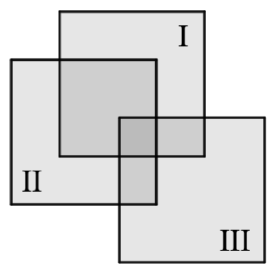
\includegraphics[max width=\textwidth, alt={Три припокриващи се еднакви квадрата I, II и III}, center]{assets/5-2-solution-figure.png}

Общата част на трите квадрата е квадрат с лице 9 cm$^2$, т.е. със страна 3 cm. Тогава общата част на I и III и на II и III е правоъгълник със страни 3 cm и $10-3=7$ cm.

(1 точка)

Страната на всеки от трите квадрата е $8+4=12$ cm.

(1 точка)

За да получим лицето на фигурата, трябва от сбора на лицата на трите квадрата $3\cdot144=432$ cm$^2$ да извадим общите части на всеки два от тях $(64+21+21=106$ cm$^2)$ и да добавим лицето на общата част на трите $(9$ cm$^2)$. Получаваме $432-106+9=335$ cm$^2$.

(2 точки)

Обиколката на фигурата е равна на обиколката на квадрат със страна $12+12-3=21$ cm, т.е. е равна на 84 cm.

(1 точка)

Задача 5.3. Три зайчета, Бън, Кей и Чип, живеят в къщичка в гората и всеки ден се разхождат по горска пътека. Те скачат с еднакви по дължина подскоци и по пътя си оставят камъчета. Бън оставя по едно бяло камъче на всеки девети подскок, Кей – по едно кафяво камъче на всеки 15-ти подскок, но ако там вече има оставено камъче, той оставя допълнително по още едно, а Чип – по едно червено камъче на всеки 6-ти подскок, но ако там вече има камъчета, ги взема и не оставя нищо. Един ден първо Бън излязъл от къщи, след него Кей и накрая Чип. На излизане всяко зайче имало по 100 камъчета и когато свършвало своите камъчета, то се връщало вкъщи.

а) На колко скока от къщи се е отдалечило всяко зайче?

б) Колко бели и кафяви камъчета е имал Чип накрая?

Решение. а) Бън се е отдалечил на $9\cdot100=900$ подскока от дома си.

Тъй като $\operatorname{НОК}(9,15)=45$, на всеки 45-ти подскок до 900-ия, Кей ще оставя по едно камъче повече. Кей ще остави $900:15+900:45=60+20=80$ от своите камъчета до 900-ия подскок. Останалите 20 камъчета ще остави за $20\cdot15=300$ подскока. Следователно Кей ще се е отдалечил на 1200 подскока от дома си.

(1 точка)

Тъй като $\operatorname{НОК}(6,9)=18$, $\operatorname{НОК}(6,15)=30$ и $\operatorname{НОК}(6,9,15)=90$, във всяка поредица от 90 подскока Чип ще оставя камъчета на всеки подскок, кратен на 6 $(90:6=15$ общо$)$, но некратен на 18 или 30. До 90-ия подскок кратните на 18 или 30 са $90:18+90:30-90:90=7$. Следователно за 90 подскока Чип ще остави $15-7=8$ камъчета.

До 900 има 10 групи от 90 подскока, т.е. Чип ще остави $8\cdot10=80$ от своите камъчета.

От 900 до 1200 подскок Чип ще оставя камъче на всеки кратен на 6 подскок с изключение на тези, които са кратни на 30.

Следователно на всяка поредица от 30 подскока ще оставя 4 камъчета.

Той има останали 20 камъчета. Следователно ще направи 5 поредици от 30 подскока. Последното си камъче Чип ще остави на $900+5\cdot30-6=1044$-тия си подскок.

(3 точки)

б) Чип е вземал по 1 бяло камъче при всеки подскок, кратен на 18 и не по-голям от 900, т.е. е взел $900:18=50$ бели камъчета.

(1 точка)

До 900-тия подскок включително Чип е вземал по 1 кафяво камъче при всеки подскок, кратен на 30 и по едно допълнително при всеки подскок, кратен на 90, общо $900:30+900:90=30+10=40$ кафяви камъчета.

От 900-ия до последния 1044 подскок Чип е вземал по 1 кафяво камъче на всеки подскок, кратен на 30, т.е. $(1020-900):30=4$ кафяви камъчета. Общо ще има 44 кафяви камъчета.

(2 точки)

Задача 5.4. В един клас всички деца са с различен ръст. Един ден всяко момче почерпило с бонбон всички ученици, които са по-високи от него, а всяко момиче почерпило с бонбон всички ученици, които са по-ниски от него.

Колко са учениците от класа, ако накрая се оказало, че:

а) две от децата не са получили бонбони, момичетата получили общо 55 бонбона, а момчетата получили общо 91 бонбона;

б) всички деца са получили по 14 бонбона?

Решение. а) Нека $D$ е най-високото момиче и $M$ е най-ниското момче.

Ясно е, че $D$ няма да получи бонбон от нито едно момиче, а всички момичета ще получат от $D$. Също, $M$ няма да получи бонбони от нито едно момче, а всички момчета ще получат от него. С нито един бонбон могат да останат само $D$ и $M$, и то само ако $M$ е по-висок от $D$. Тогава и $M$ няма да получи бонбон от нито едно момиче.

(2 точки)

Ако момичетата, по-ниски от $D$, са $n$ на брой, а момчетата, по-високи от $M$, са $m$ на брой, то учениците са подредени във възходящ ред така:

$$\text{момиче}_1,\ \text{момиче}_2,\ \ldots,\ \text{момиче}_n,\ D,\ M,\ \text{момче}_1,\ \text{момче}_2,\ \ldots,\ \text{момче}_m.$$

Момичетата са получили общо $n+(n-1)+\cdots+1=55$ бонбона. Тъй като $1+2+\cdots+10=55$, то $n=10$.

Аналогично момчетата са получили общо $1+2+\cdots+m=91$ бонбона. Тъй като $1+2+\cdots+13=91$, то $m=13$. Следователно учениците са $10+13+2=25$.

(2 точки)

б) Нека всички деца са подредени по височина и $A$ и $B$ са две съседни деца, като $A$ е по-ниско от $B$. Ако $A$ и $B$ са две момчета, то те ще получат по равен брой бонбони от останалите деца, но $B$ ще получи от $A$, т.е. ще има 1 бонбон повече от $A$. Ако $A$ и $B$ са две момичета, то $A$ ще получи от $B$, т.е. $A$ ще има с 1 бонбон повече от $B$. Ако $A$ е момче, $B$ е момиче, то те получават еднакъв брой бонбони от всички останали и си разменят по 1 бонбон. Следователно $A$ и $B$ получават еднакъв брой бонбони. Ако $A$ е момиче, $B$ е момче, то те получават еднакъв брой бонбони от всички останали и не си разменят бонбони помежду си. Следователно отново получават еднакъв брой бонбони.

За да получат всички деца по 14 бонбона, в редицата се редуват момче и момиче във възходящ ред.

(1 точка)

Ако най-ниското дете е момче, то е получило бонбони само от всички момичета, следователно момичетата са 14.

Ако най-ниското дете е момиче, то е получило бонбони само от останалите момичета и от нито едно момче. Следователно момичетата са 15.

Ако най-високото дете е момиче, то е получило бонбони само от всички момчета, следователно момчетата са 14.

Ако най-високото дете е момче, то е получило бонбони само от останалите момчета, следователно момчетата са 15.

Тези случаи могат да се обобщят в таблица:

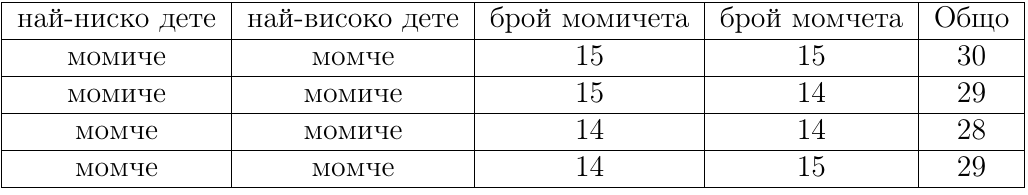
\includegraphics[max width=\textwidth, alt={Таблица на четирите случая според пола на най-ниското и най-високото дете}, center]{assets/5-4-solution-table.png}

Следователно броят на децата в класа е 28, 29 или 30.

(2 точки)
